\chapter{Grundlagen}
\section{Historie}
Seit dem Beginn des Industriezeitalters um 1800, welches mit der Mechanisierung (Industrie 1.0) startete, befindet sich die Industrie in einem stetigen Wandel. Sie entwickelte sich um 1900 durch die Massenproduktion zur Industrie 2.0 und in den 1970er Jahren durch die Automatisierung zur Industrie 3.0. Die Einteilung der Industriezeitalter ist durch tiefgreifende Veränderungen im technologischen Fortschritt möglich, welche auch als industrielle Revolution bezeichnet werden. Aktuell befinden wir uns in der Phase der 4. industriellen Revolution.

Die 1. industrielle Revolution fand mit der Erfindung der Dampfmaschine statt. Sie ermöglichte es Eisenbahnen und Dampfschiffe sowie verschiedene Maschinen im Kohleabbau oder in Textilfabriken anzutreiben und trug massiv zur Industrialisierung und der Entstehung der Industrie 1.0 bei. Nach und nach wurden immer mehr Produktionsanlagen errichtet und somit Arbeitsplätze in Infrastruktur, Textilfabriken, Häuserbau, Kohleabbau und anderen Bereichen geschaffen.

Die Erforschung der Elektrizität im 19. Jahrhundert war der Auslöser der 2. industriellen Revolution. Nachdem ab 1830 die Gesetze der Elektrotechnik bekannt waren, fand die Elektrizität eine breite Anwendung in der Industrie und im Alltag. Im Jahr 1913 führte Henry Ford das Fließband in der Automobilbranche ein. Im Zuge dessen musste jeder Arbeiter nur noch einen Arbeitsschritt erledigen, welches einerseits die Produktion wesentlich beschleunigte und eine Massenproduktion ermöglichte und andererseits eine hohe Spezialisierung der einzelnen Arbeitskräfte für ihre bestimmten Aufgaben erforderte. Außerdem wurde es durch die Luftfahrt möglich Produkte wie Autos, Kleidung und Lebensmittel über Kontinente hinweg immer schneller zu transportieren und zu handeln.

Die 3. industrielle Revolution fand in den 1970er Jahren statt. Sie ist durch eine sukzessive (Teil-) Automatisierung der Prozesse und durch den Einzug der IT in die Industrie- und Verbraucherwelt geprägt. In den 1940er Jahren wurden die ersten Rechenmaschinen und programmierbare Steuerungen in Unternehmen eingesetzt. In den 1970er Jahren zog der Computer auch in den Privatbereich ein, wurde zunehmend beliebter und schaffte einen neuen Industriezweig. Der Fertigungsprozess in Fabriken wurde mehr und mehr von Maschinen übernommen. Durch den zunehmenden Einsatz von IT in Unternehmen entstand immer mehr Kommunikation zwischen Menschen und Maschinen. Diese Kommunikation und die anfallenden Daten wurden jedoch nur unternehmensintern verarbeitet. Es gab nur wenige Schnittstellen nach außen.

Das Ende des 20. Jahrhunderts gilt als der Beginn der 4. industriellen Revolution. Das Kennzeichen dieser Phase ist die zunehmende Digitalisierung und der Einzug der Internet-Technologien in die Industrie. Mit ihr geht die technische Vernetzung physischer Gegenstände, dem \ac{IoT}, einher. Mehr und mehr Geräte oder Gegenstände besitzen die Möglichkeit aktiv über eine Netzwerkschnittstelle, oder passiv mit Hilfe eines Bar- oder QR-Codes mit der digitalen Welt zu kommunizieren und somit eine fortschreitende Automatisierung und Individualisierung zu ermöglichen. Diese Entwicklung macht es möglich immer schneller Informationen auszutauschen, größere Datenmengen zu analysieren und diese zu verarbeiten. In der Industrie entstehen dadurch u. a. die folgenden Chancen:

\begin{itemize}
  \item Die Kommunikationsinfrastruktur wird in Zukunft in Produktionssystemen so preiswert sein, dass sie sinnvoll für Konfiguration, Service, Diagnose, Bedienung und Wartung genutzt werden kann.
  \item Die Produktionssysteme werden mehr und mehr mit einem Netz verbunden, erhalten dort eine digitale Identität, werden somit such- und analysierbar und besitzen die Möglichkeit Daten über sich selbst zu veröffentlichen. 
  \item Maschinen und Anlagen speichern ihre Zustände in ihrer digitalen Identität im Netz. Diese Zustände sind aktuell, aktualisierbar und zunehmend vollständig. Sind im Netzwerk viele solcher Identitäten vorhanden, können die Daten effizient abgerufen und ausgetauscht werden.
  \item Softwaredienste werden über das Netz verknüpft und können somit automatisiert individuelle Aufgaben durch die direkte Kommunikation der Systeme erledigen. Eine solche individuelle Wertschöpfung war bisher nur unwirtschaftlich oder gar nicht möglich.
\end{itemize}

Im Gegensatz zur Industrie 3.0 sollen Maschinen autonom, auch über Unternehmensgrenzen hinweg, miteinander kommunizieren können um gesamte Geschäftsprozesse zu übernehmen. Dies setzt eine Öffnung der Unternehmen nach außen voraus und wird in \autoref{Grundlagen:Industrie4.0-Kommunikation} dargestellt.

\begin{figure}[h]
  \centering
  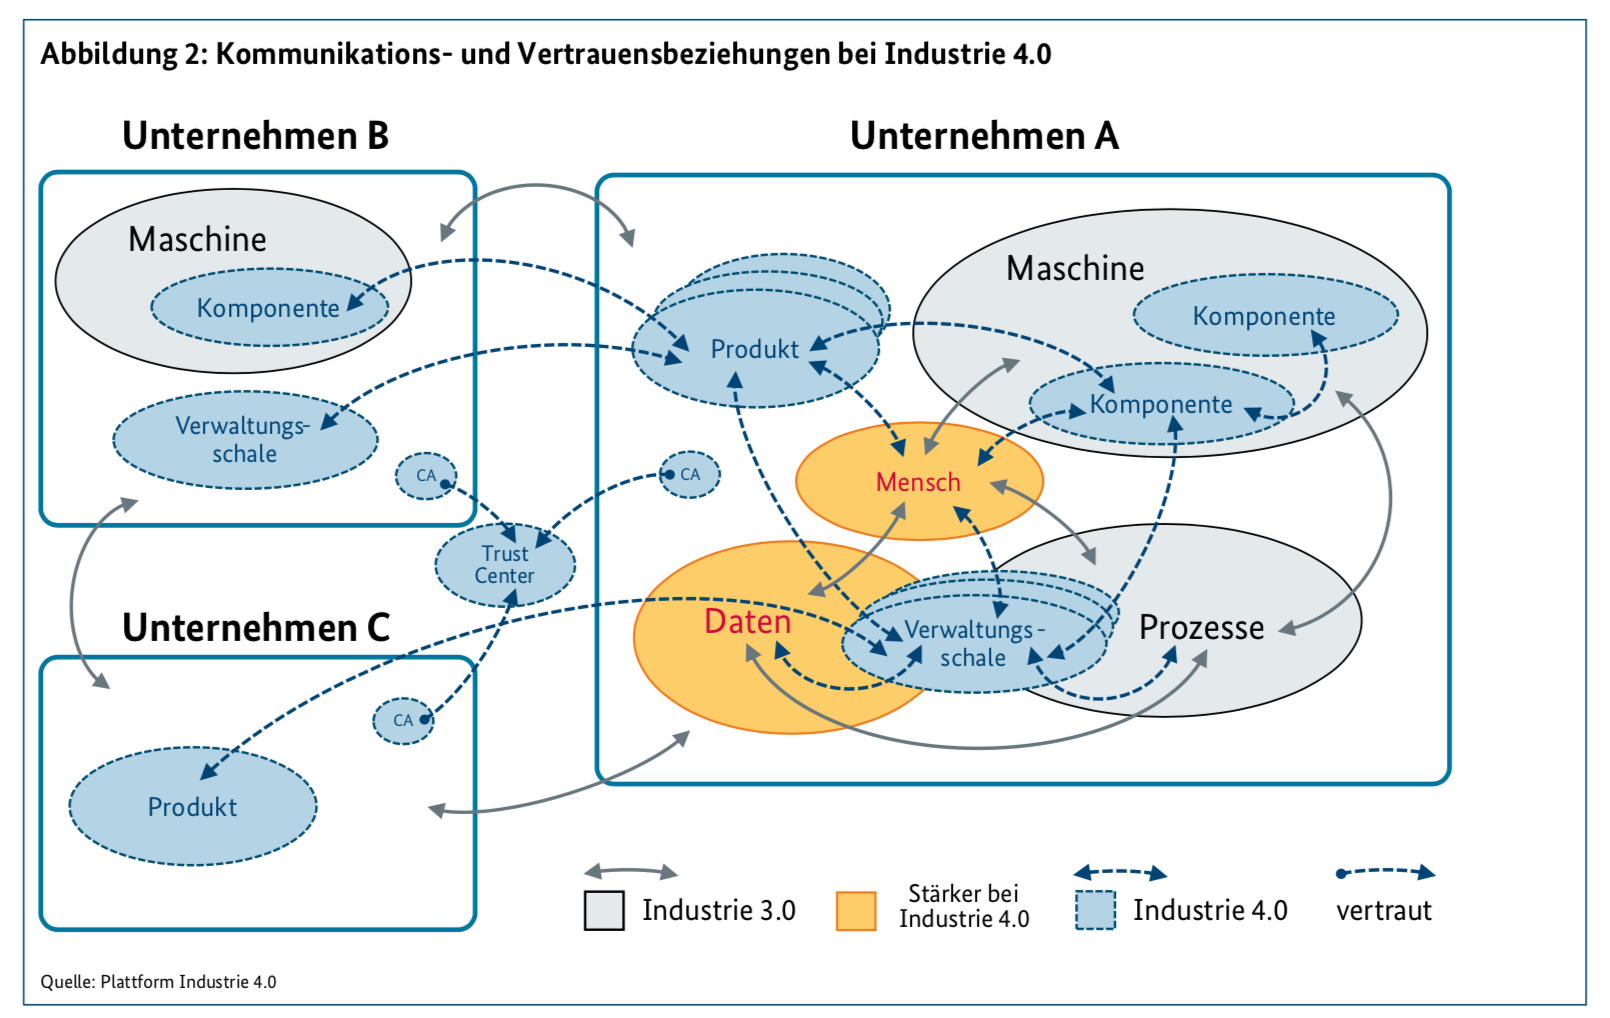
\includegraphics[width=12cm]{kommunikationsbeziehungen-i40}
  \caption{Kommunikationsbeziehungen in einer Industrie 4.0 Umgebung}
  \label{Grundlagen:Industrie4.0-Kommunikation}
\end{figure}

\clearpage

\section{Automatisierungspyramide}
\label{Grundlagen:Automatisierungspyramide}
Die Automatisierungspyramide (\autoref{Grundlagen:Automatisierungspyramide-img}) stellt die beteiligten Systeme und Softwarekomponenten eines automatisierten Prozesses dar. In der Industrie 4.0 wird eine automatisierte und direkte Kommunikation zwischen allen Ebenen der Automatisierungspyramide angestrebt. Die beteiligten Systeme beginnen, ausgehend vom Kundenauftrag und der betriebswirtschaftlichen Planung der Produktion auf der Unternehmensebene beim \ac{ERP} System. Die Ergebnisse der Planung werden an das \ac{MES} übergeben, welches die verschiedenen Fertigungs- oder Logistikaufträge generiert. Die Aufträge werden anschließend auf der Prozessleit- (\ac{SCADA}), Steuerungs- (\ac{SPS}) und Feldebene (Ein-/Ausgangssignale) mit Hilfe von Steuerungen und Sensoren bearbeitet. Während die oberen Schichten der Pyramide (\ac{ERP} und \ac{MES}) durch Standardkomponenten bzw. -software der IT realisiert werden, zählen die unteren Schichten (Prozessleit- bis Feldebene) zur Automatisierung, welche die Steuerung und Kontrolle der technischen Anlagen übernimmt. Sie sind durch spezielle Hard- und Softwarelösungen umgesetzt. Die Integration von Sicherheitsmaßnahmen bei der Kommunikation dieser Systeme stellt oft eine große Herausforderung dar, da besondere Anforderungen vorliegen oder wenig Ressourcen zur Verfügung stehen. (\cite{Sander2014})

\begin{figure}[h]
  \centering
  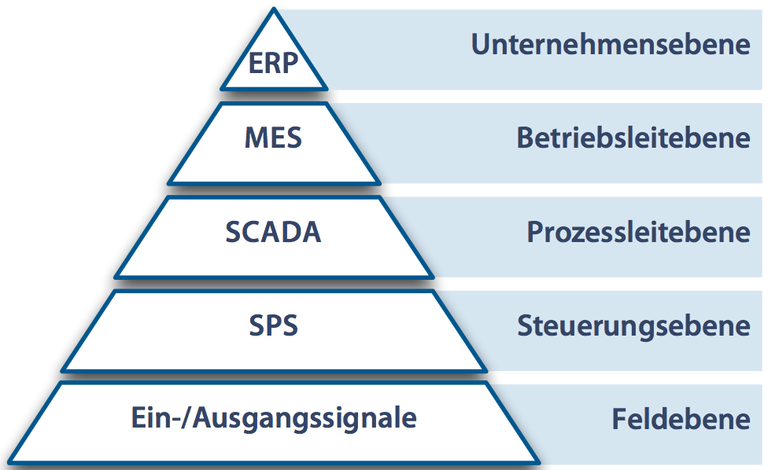
\includegraphics[width=10cm]{automatisierungspyramide}
  \caption{Automatisierungspyramide}
  \label{Grundlagen:Automatisierungspyramide-img}
\end{figure}

\section{Industrie 4.0}
Der Begriff Industrie 4.0 wurde erstmals auf der Hannover Messe 2011 verwendet (\cite{drath2014}) und soll das Ergebnis der 4. industriellen Revolution darstellen. Der Grundgedanke hinter Industrie 4.0 ist die flächendeckende Vernetzung von Informations- und Kommunikationstechnik zu einem Internet der Dinge, Dienste und Daten (\cite{spath2013}). Diese Vernetzung soll einen ständigen Informationsaustausch zwischen den Komponenten ermöglichen. Jede Komponente des \ac{IoT} soll als \ac{CPS} arbeiten. Ein \ac{CPS} besitzt neben seiner realen Identität eine digitale Identität, über welche es ständig mit anderen \ac{IoT}-Geräten kommunizieren kann. Kunden- und Maschinendaten werden miteinander vernetzt (\cite{rami2016}). Dieser Prozess beschreibt auch einen Wandel in der Strukturierung und Organisation der Produktion in Unternehmen. Durch die fortschreitende Automatisierung wird die Umsetzung einer immer höheren Individualisierung bei geringerer produzierter Stückzahl rentabel. \autoref{Grundlagen:Das Internet der Dinge} zeigt die Vernetzung der verschiedenen Industriesektoren und Komponenten über das \ac{IoT}.

\begin{figure}[h]
  \centering
  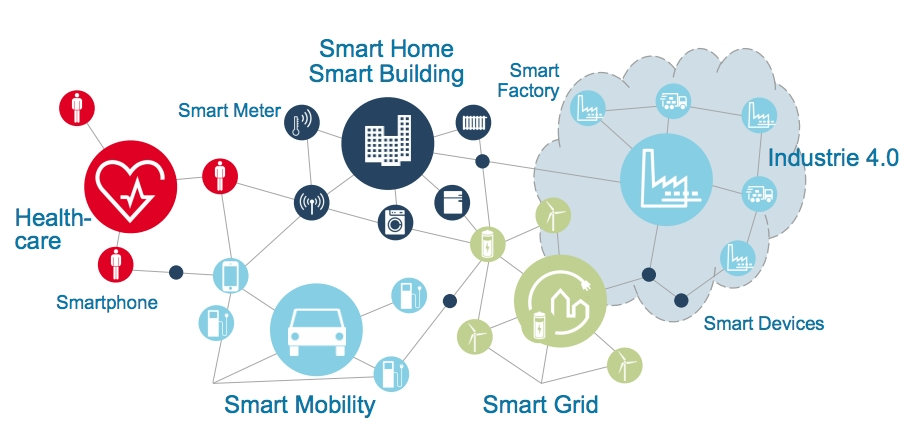
\includegraphics[width=12cm]{internet-der-dinge}
  \caption{Das Internet der Dinge}
  \label{Grundlagen:Das Internet der Dinge}
\end{figure}

\subsection{Internet of Things/Industrial Internet of Things}
\label{Grundlagen:IoT/IIoT}
Die fortschreitende Vernetzung der Komponenten spiegelt sich im \ac{IoT} bzw. \ac{IIoT} wieder. Das \ac{IoT} beschreibt im Gegensatz zum \ac{IIoT} ein verbraucherorientiertes Konzept für die Nutzung von digitalisierten und vernetzten Systemen. Hierbei werden die physischen Systeme virtuell abgebildet. Dies wird genutzt, um die Effektivität der Systeme zu verbessern und intelligente Services zu nutzen.

Das \ac{IoT} ist ein wesentlicher Bestandteil der Industrie 4.0, welche Netzwerke aus Systemen, Daten und Dienstleistungen herstellt, in denen diese Komponenten miteinander kommunizieren. Im Verbraucherbereich und für die Kommunikation zwischen Mensch und Maschine findet das Protokoll \ac{HTTP} und dessen \ac{REST} Programmierparadigma breite Anwendung. 

Das \ac{IIoT} beschreibt den Gebrauch von \ac{IoT}-Technologien im industriellen Raum. Diese Systeme können besondere Anforderung an die Kommunikation im Netzwerk wie Skalierbarkeit, Ressourcenverbrauch, Echtzeitkommunikation oder Sicherheit stellen. Des Weiteren findet in Industrie 4.0 Umgebungen \ac{M2M} Kommunikation statt. Um diesen Problemen entgegenzuwirken, wurden neue Protokolle zur Übermittlung von Daten im Netzwerk entwickelt. Hierbei erfahren vor allem die Protokolle \ac{MQTT} und \ac{CoAP} ein hohes Maß an Beachtung. Diese Protokolle wurden für eine ressourcenschonende Kommunikation zwischen Maschinen entwickelt.

\subsection{Referenzarchitekturen}
Um eine flächendeckende Vernetzung der digitalen Komponenten zu ermöglichen, muss eine einheitliche Kommunikation geschaffen werden. Diese beschränkt sich nicht nur auf die Form der Nachrichten im Netzwerk und der Gewährleistung der Sicherheit, sondern beinhaltet auch die Struktur und Bereitstellung der Informationen im Netzwerk. In der Folge wurden verschiedene Referenzarchitekturmodelle entwickelt, um Standards für die Kommunikation und Interaktion von Netzwerkkomponenten innerhalb einer Industrie 4.0 Umgebung zu definieren.

\subsubsection{\ac{RAMI4.0}}
\label{Grundlagen:RAMI4.0}
Das \ac{RAMI4.0} wird in der DIN SPEC 91345 beschrieben und dient als Konzept zur strukturierten Umsetzung der grundlegenden Idee hinter dem Begriff Industrie 4.0. Die Aufgabe des Architekturmodells ist es, die Ziele einer Industrie 4.0 Umgebung, die vollständige Vernetzung der physischer Wertgegenstände, umzusetzen. Diese Gegenstände werden im Rahmen der \ac{RAMI4.0} als \textit{Assets} bezeichnet. Jedes \textit{Asset} besitzt seine eigene Verwaltungsschalte, welche als Schnittstelle zum Austausch von Informationen dient. Die Verwaltungsschale soll eine standardisierte Kommunikation und einfache Inbetriebnahme neuer Komponenten ermöglichen (\cite{rami2016}). Mit Hilfe der \ac{RAMI4.0} soll es möglich sein, den Status eines \textit{Assets} zu jedem Zeitpunkt im Lebenszyklus nachweisen zu können. Die \ac{RAMI4.0} ist in \autoref{Grundlagen:RAMI4.0-img} dargestellt und wird durch ein Modell aus sechs Schichten und drei Achsen dargestellt. (\cite{RAMISpec})

Auf der Architekturachse werden sechs Schichten beschrieben. Auf der untersten Schicht wird der Gegenstand der physischen Welt dargestellt. Alle zu ihm relevanten Information werden in den darüberliegenden Schichten gespeichert. Darüber stellt die \textit{Integration} Schicht das Bindeglied zwischen der physischen und digitalen Welt bereit, indem sie die Eigenschaften des \textit{Assets} für Computersysteme erreichbar macht (\cite{BMWiNeCon2016}). Die \textit{Communication} Schicht beschreibt den Zugriff auf die Ressourcen und Funktionen der Komponente und stellt die Dienste einer \ac{SOA} bereit. Auf der \textit{Information} Schicht wird die Funktionalität des \textit{Assets} gespeichert und die Datenintegrität gewährleistet. Die \textit{Functional} Schicht beschreibt die Form, wie und mit welchen Parametern ein Funktionsaufruf stattfinden kann. In der \textit{Business} Schicht werden die geschäftsrelevanten Daten gehalten. (\cite{RAMISpec})

Die Hierarchieachse zeigt die Anlagen, Maschinen sowie das Endprodukt, welche miteinander vernetzt sind. Die in \autoref{Grundlagen:Automatisierungspyramide} beschriebene Automatisierungspyramide findet sich in der Hierarchieebene der \ac{RAMI4.0} wieder. Sie wurde dort auf der niedrigsten Ebene um das Produkt (\textit{Product}) sowie auf der höchsten Ebene um die Stufe \textit{Connected World} erweitert. Die \textit{Connected World} beschreibt den Zusammenhang zwischen einem Asset oder einer Assetkombination und einem anderen Asset oder einer Assetkombination, also einem Fabrikverbund. (\cite{RAMISpec})

Der Produktlebenszyklus wird im Gegensatz zur Industrie 3.0 in das Netzwerk mit eingebunden. Der gesamte Prozess der Produktion, Wartung bis hin zur Verschrottung wird digital erfasst. Somit könnten ständig Informationen über vorhandene \textit{Assets} gesammelt und zur Optimierung des Werschöpfungsprozesses analysiert werden. (\cite{RAMISpec})

\begin{figure}[h]
  \centering
  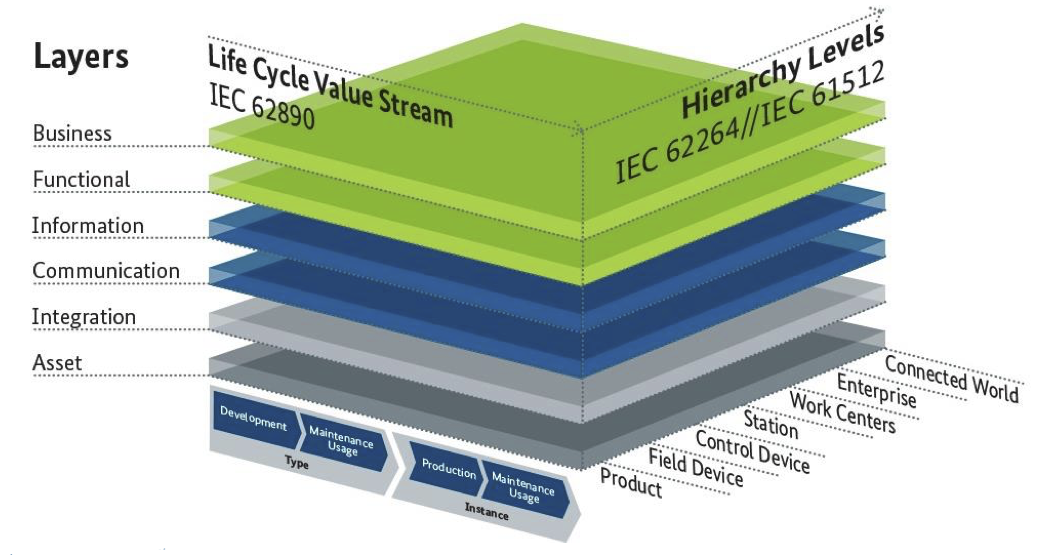
\includegraphics[width=12cm]{rami40}
  \caption{RAMI 4.0}
  \label{Grundlagen:RAMI4.0-img}
\end{figure}

\subsubsection{IIRA}
\label{Grundlagen:IIRA}
Das \ac{IIC} veröffentlichte im Jahr 2015 die \ac{IIRA}. Die \ac{IIRA} beschreibt eine standardbasierte, offene Referenzarchitektur für \ac{IIoT}, welches auf dem \ac{IIAF} basiert. Das \ac{IIAF} unterstützt die Unternehmen bei der Entwicklung, Dokumentation, Kommunikation und Bereitstellung von Systemen im \ac{IIoT} Bereich (\cite{iira2017}). Die Beschreibung der Architektur findet mit einem hohen Maß an Abstraktion statt, um das breite Feld der verschiedenen Industrielösungen abdecken zu können und standardisierte Vorgehensweisen zu ermöglichen. Das \ac{IIAF} folgt der Vorgehensweise des ISO/IEC/IEEE Standard 42010:2011\footnote{ISO/IEC/IEEE Standard 42010:2011 - Systems and Software Engineering–Architecture Description}. Hieraus werden die grundlegenden Architekturbeschreibungskonstrukte \textit{Concern}, \textit{Stakeholder} und \textit{Viewpoint} übernommen. Die \textit{Viewpoints} sind die grundlegenden Ebenden beim Aufbau der \ac{IIRA}. Dabei werden vier \textit{Viewpoints} für die Beschreibung festgelegt. Die Struktur der \ac{IIRA} und deren \textit{Viewpoints} wird in \autoref{Grundlagen:IIAF/IIRA - Übersicht} dargestellt. (\cite{heidrich2016})

Der \textit{Business Viewpoint} beinhaltet die betriebswirtschaftlichen \textit{Concerns} bei der Umsetzung eines \ac{IIS} sowie die entstehenden Rahmenbedingungen. Es werden die Systemeigenschafen definiert, welche an die Geschäftsziele gekoppelt sind. Die \textit{Stakeholder} dieses \textit{Viewpoints} bestehen aus Führungskräften, Produktmangern und Systemingenieuren.

Im \textit{Usage Viewpoint} werden die \textit{Concerns} bei der Nutzung eines \ac{IIS} beschrieben. Dies beinhaltet die Beschreibung der Bedienabläufe.

Der \textit{Functional Viewpoint} beschreibt die funktionalen Komponenten des \ac{IIS}. Es werden Zusammenhänge, Struktur, Schnittstellen und Interaktionen mit Systemen im Netzwerk sowie der Außenwelt beschrieben.

Der \textit{Implementation Viewpoint} beinhaltet die Technologien zur Umsetzung des \ac{IIS}. Es werden die funktionalen Komponenten, deren Vernetzung, Kommunikationsschnittstellen sowie deren Produktlebenszyklen dargestellt. Diese \textit{Concerns} sind wichtige Ansatzpunkte für Komponentendesigner, Systementwickler und Integratoren. 

\begin{figure}[h]
  \centering
  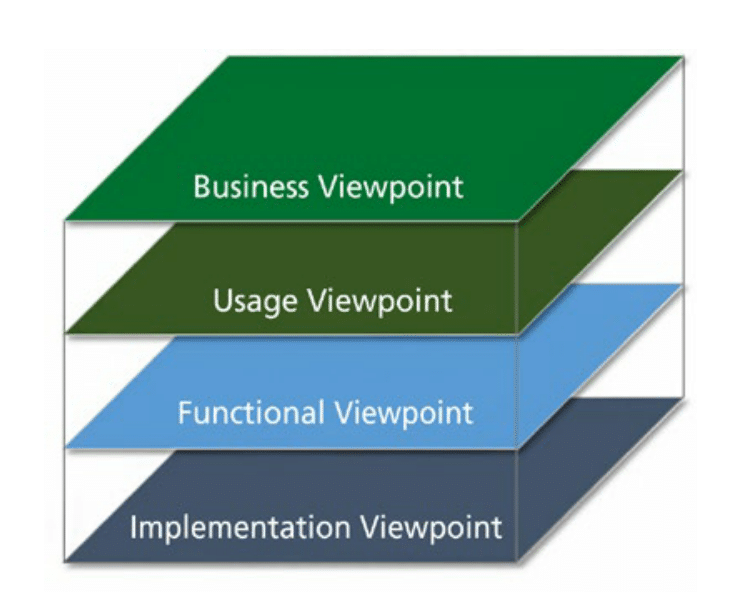
\includegraphics[width=10cm]{iira}
  \caption{Die Grundebenen der IIRA} 
  \label{Grundlagen:IIAF/IIRA - Übersicht}
\end{figure}

Die Anforderungen des Referenzarchitekturmodells beinhalten niedrige Latenzen und Schwankungen, einen hohen Durchsatz, Skalierbarkeit, Ausfallsicherheit, Datensicherheit und \ac{QoS}. Die \ac{IIRA} stellt einen softwaretechnischen Ansatz der Darstellung einer Referenzarchitektur bereit.

\subsection{Kommunikationsstrukturen}
\label{Grundlagen:Kommunikationsstrukturen}
Da die grundlegende Netzwerkstruktur der vorhandenen Netze, welche auf \ac{IP} basieren, für die Industrie 4.0 weiterhin genutzt werden sollen, kann davon ausgegangen werden, dass auch in Zukunft der wesentliche Teil der Kommunikation mit Hilfe des \ac{TCP}/\ac{IP} Referenzmodells stattfinden wird. Die Transportprotokolle \ac{TCP} und \ac{UDP} basieren auf dem Protokoll \ac{IP}. Sie er möglichen es Daten, je nach Anforderungen, zuverlässig oder unzuverlässig im Netzwerk zu verteilen. Hierbei muss ein Augenmerk auf die Sicherheit der Kommunikation und deren Effizienz gelegt werden. Das verwendete Anwendungsprotokoll sowie der genutzte Kommunikationsstack müssen entsprechende Sicherheitsmechanismen bereitstellen, um eine Identifikation und Authentifizierung des Kommunikationspartners durchzuführen. (\cite{sichKom2017})

\subsubsection{End2End}
\label{Grundlagen:End2End}
Die Komponenten der Industrie 4.0 Umgebung können mit Hilfe des Protokolls \ac{TCP} über einen direkten Kanal miteinander kommunizieren. Dies setzt voraus, dass sich beide Teilnehmer in einem Netzwerk befinden, welches die benötigten Dienste zur Herstellung der Verbindung bereitstellt. Anschließend können die in der Verwaltungsschale gespeicherten Informationen über die logischen Schnittstellen im Netzwerk verfügbar gemacht werden und zwischen den Komponenten ausgetauscht werden.

\subsubsection{Gateways}
Damit bereits existierende Systeme in die Industrie 4.0 Welt überführt werden können, werden Gateways genutzt, welche eine Industrie 4.0 konforme Kommunikation dieser Systeme bereitstellen. In der Industrie sind Systeme vorhanden, welche keine Ressourcen oder Schnittstellen für die Umsetzung einer Industrie 4.0 konformen Kommunikation haben oder aus Gründen der Leistungsoptimierung proprietäre Protokolle nutzen. Die Gateways müssen auf diese Systeme und deren Protokolle individuell konfiguriert werden, um die Übersetzung der Kommunikation bereitstellen zu können.

Durch die Nutzung von Gateways können die Systeme im Netzwerk in verschiedene Domänen getrennt werden und der Datenfluss an zentraler Stelle kontrolliert und analysiert werden.

\subsubsection{Publish-Subscribe}
\label{Grundlagen:Publish-Subscribe}
Das Publish-Subscribe Modell bietet die Möglichkeit Informationen an mehrere Teilnehmer zu verteilen. Hierbei melden sich die Empfänger beim Verteiler an und wählen aus, über welche Nachrichtentypen sie informiert werden möchten. Diese Verteildienste nutzen zur besseren Skalierung und Reduzierung der Netzlast das Datagramm \ac{UDP}. Durch die Nutzung dieses Transportprotokolls geht die Fehlertoleranz während der Übertragung verloren. Es muss entweder dafür gesorgt werden, dass eine zuverlässige Netzwerkinfrastruktur vorhanden ist und hohe Bandbreitenreserven geschaffen werden, um die Dienstgüte (\ac{QoS}) sicherzustellen oder dieses Modell nur für fehlertolerante Kommunikation wie z. B. Audio- und Video-Anwendungen zu nutzen.

\subsubsection{Kommunikation mit Netzwerk als Partner}
Zeitkritische Automatisierungsanwendungen verlangen besondere Netzwerkeigenschaften. Sie können auf geringe Latenzen oder Jitter angewiesen sein. Um diese Eigenschaften sicherzustellen, ist es sinnvoll in diese Netze eine Industrie 4.0 Schnittstelle zu integrieren. Somit ist es den Teilnehmern möglich, über die Verwaltungsschale der Schnittstelle im Netzwerk sicherzustellen, dass das Netzwerk die erforderlichen Anforderungen bereitstellt. (\cite{sichKom2017})

\subsection{Protokolle}
Die Kommunikation in Industrie 4.0 Umgebungen findet nicht mehr über einzelne, vorgegebene Schnittstellen der verschiedenen Ebenen der Automatisierungspyramide statt, sondern direkt von den Produktionssystemen. Um dies zu ermöglichen, ist es notwendig, eine einheitliche Kommunikation durch Normen und Standards herzustellen. Durch die in der Industrie 4.0 benötigte \ac{M2M} Kommunikation wurde die Entwicklung neuer Protokolle zum effizienten Informationsaustausch vorangetrieben, welche es ermöglichen sollen, eine Standardisierung bereitzustellen und somit eine herstellerübergreifende und plattformunabhängige Kommunikation zu ermöglichen. Hierbei haben sich bzgl. der Referenzarchitekturen \ac{RAMI4.0} und \ac{IIRA} die Protokolle \ac{OPC UA} und \ac{DDS} etabliert.

\subsubsection{\ac{OPC UA}}
\ac{OPC UA} ist in der \ac{IEC} 62541\footnote{IEC 62541 - OPC Unified Architecture} als offener Standard definiert und erstreckt sich über die Schichten \textit{Communication} und \textit{Information} des \ac{RAMI4.0}. Es vereint Daten- und Informationsdienste und stellt einen sicheren, zuverlässigen und plattformübergreifenden Informationsaustausch zwischen unterschiedlichen Geräten und Systemen der Industrie bereit. Die \ac{OPC UA} ermöglicht die Kommunikation über die verschiedenen Schichten der Automatisierungspyramide von der Feldebene bis zur Unternehmensebene. 

\ac{OPC UA} stellt ein Informationsmodell mit Hilfe einer \ac{SOA} bereit, erfüllt die Anforderungen des \ac{RAMI4.0}, etabliert sich zunehmend im Maschinen- und Anlagenbau und bietet einen vielversprechenden Ansatz für einen standardisierten Informationsaustausch über Unternehmensgrenzen hinweg (\cite{OPCWegbereiter2014}). Aufgrund dessen stellt es auch ein attraktives Ziel für Industriespionage und die Sabotage von Industrienetzen bereit (\cite{opcpt2}).

\ac{OPC UA} wird in 14 geschichteten Spezifikationen beschrieben, welche sich in die Bereiche \textit{Core}, \textit{Access Type} und \textit{Utility} unterteilen lassen. Dabei stellen die Spezifikationen 1-7 sowie 14 die Kernfunktionalitäten des Architekturmodells dar. Sie beschreiben die Struktur des OPC Addressraums und der Dienste, die darauf operieren. Die Spezifikationen 8-11 wenden diese Kernfunktionalitäten auf spezifische \ac{OPC COM} Spezifikationen, wie \ac{DA}, \ac{AE} und \ac{HDA} an. Die Teile 12 und 13 beinhalten Mechanismen zur Discovery von Systemen und beschreiben Möglichkeiten der Datenaggregation. Eine Übersicht der \ac{OPC UA} Spezifikation wird in \autoref{Grundlagen:OPC UA Spezification} dargestellt.

\begin{figure}[h]
  \centering
  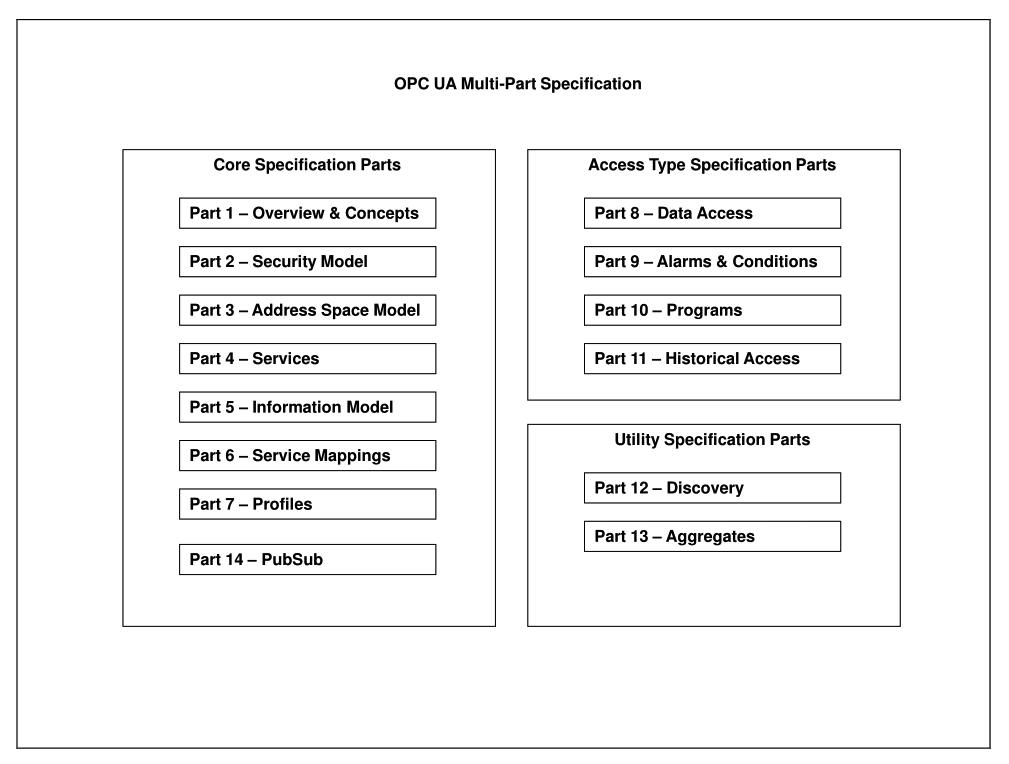
\includegraphics[width=12cm]{opcua-spezifikation}
  \caption{OPC UA Spezifikation} 
  \label{Grundlagen:OPC UA Spezification}
\end{figure}

Das Lesen- und Schreiben von Daten und die Kommunikation in Industrie 4.0 Umgebungen findet nach \ac{RAMI4.0} durch die Verwaltungsschale der Komponenten statt. Diese wird im \ac{OPC UA} Stack durch den Adressraum beschrieben. Der Adressraum wird zur Speicherung von Knoten, deren Attribute und Referenzen zu anderen Knoten genutzt. Der Addressraum und das Informationsmodell von \ac{OPC UA} werden in den Spezifikationen 3 \cite{opcpt3} und 5 \cite{opcpt5} definiert.

\ac{OPC UA} ermöglicht die Kommunikation der Assets über ein Client-Server Pattern. Die Architektur setzt sich dabei aus einem \ac{OPC UA} Client und einem \ac{OPC UA} Server zusammen. Der \ac{OPC UA} Server stellt verschiedene Funktionen bereit, auf welche der \ac{OPC UA} Client mit Hilfe eines Request zugreifen kann. Des Weiteren ist es möglich durch einen Request des \ac{OPC UA} Clients ein Element des Servers beobachten zu lassen, um bei Änderungen vom Server benachrichtigt zu werden. Um die Kommunikation zwischen \ac{OPC UA} Servern zu gewährleisten, wird ein \ac{OPC UA} Client in einen \ac{OPC UA} Server integriert. In der Grafik \autoref{Kap2:OPC UA Client-Server Architektur} wird das Client-Server Pattern der \ac{OPC UA} Spezifikation schematisch dargestellt. Die linke Seite der Grafik beschreibt die Kommunikation zwischen einem Client und einem Server mit eingebettetem Client. In der rechten Seite der Grafik findet die Kommunikation zwischen dem eingebetteten Client und einem \ac{OPC UA} Server statt.

\begin{figure}[h]
  \centering
  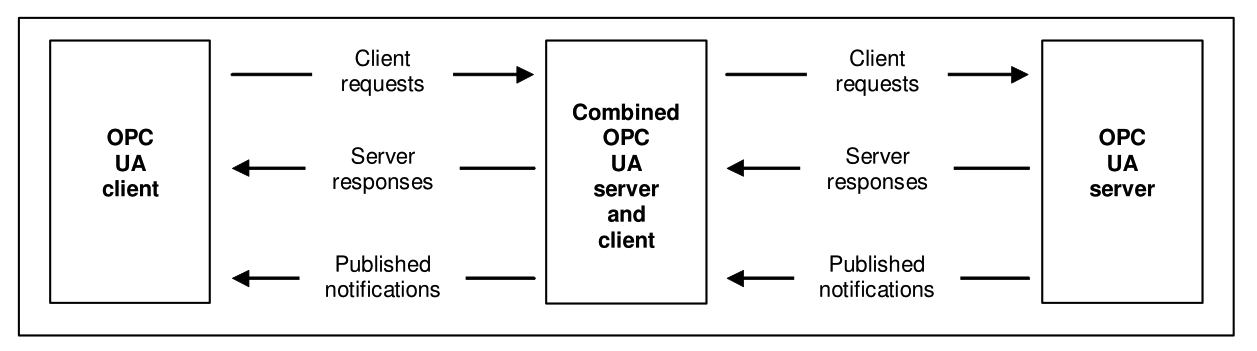
\includegraphics[width=12cm]{opcuaclient-server}
  \caption{OPC UA Client-Server Architektur}
  \label{Kap2:OPC UA Client-Server Architektur}
\end{figure}

\ac{OPC UA} wurde ursprünglich als Client-Server Architektur entwickelt. Um \ac{OPC UA} besser in Systemen der unteren Ebenen der Automatisierungspyramide, wie Kleinsteuerungen, Sensoren und Low-End /textit{embedded} Systemen, einsetzen zu können, werden meist geringe Latenzen in den Netzwerken und ein geringer Overhead aufgrund von Ressourcenmangel sowie die Kommunikation mit mehreren Partnern benötigt. Diese Anforderungen wurden von dem im Jahr 2018 veröffentlichten 14. Teil der \ac{OPC UA} Spezifikation \textit{Publish Subscribe} adressiert (\cite{hoppe2018}). Das Publish-Subscribe Modell ermöglicht die Nutzung von \ac{OPC UA} in \ac{WAN} Umgebungen und die Verwendung von Protokollen wie \ac{MQTT} und \ac{AMQP}, während die Ende-zu-Ende Sicherheit und die standardisierte Datenmodellierung erhalten bleiben. Es wird das fehlertolerante Datagramm \ac{UDP} als Transportprotokoll verwendet, wodurch geringe Latenzen bei der Kommunikation sowie Broad- und Multicast Funktionalitäten ermöglicht werden. Das \textit{Publish Subscribe} Modell bietet sich zur Übertragung von kleinen Datenmengen zum \textit{Logging} oder \textit{Monitoring} im Netzwerk an. Dabei muss das Netzwerk durch die Nutzung von \ac{UDP} nicht bei jeder Datenübertragung durch einen \ac{TCP} Verbindungsaufbau belastet werden (\cite{opcpt1}).

\subsubsection{\ac{DDS}}
\ac{DDS} ist ein weiterer offener Standard der \ac{OMG} und stellt eine \ac{MOM} zur Kommunikation in hochdynamischen verteilten Systemen dar. Er wurde für niedrige Latenzzeiten, einen hohen Datendurchsatz und eine skalierbare, belastbare und sichere Datenverteilung entwickelt, um die Kommunikation in Steuerungs- und Kontrollaufgaben zu realisieren. Der beschriebene Standard deckt alle Anforderungen der \ac{IIRA} ab und hat sich bereits in industriellen Systemen etabliert. Gegenüber \ac{OPC UA} beschreibt \ac{DDS} eine dezentralisierte Architektur. Es bietet ein Konnektivitäts-Framework, welches ein Kommunikationsparadigma basierend auf einem Shared Data Model, einen Standard für die Definition domain-spezifischer Informationsmodelle, ein starkes Sicherheitsmodell, Discovery und reichhal­tige APIs beinhaltet. Die Kommunikation findet direkt vom Publisher zum Subscriber statt. Dabei werden Latenzzeiten reduziert und durch die Nutzung von Broad- und Multicast die Netzlast beim Bereitstellen von Informationen an viele Empfänger gering gehalten. Es ist möglich die \ac{MOM} \ac{DDS} in eine \ac{OPC UA} Architektur zu integrieren und mit dem von der \ac{RAMI4.0} bereitgestellten Informationsmodell zu nutzen.

\subsection{Anforderungen an die Netzwerkkommunikation}
\label{Grundlagen:Anforderungen}
Aufgrund der unterschiedlichen Einsatzbereiche von Industrie 4.0 Systemen, unterscheiden sich auch dementsprechend deren Anforderungen. Um die Anforderungen einer Industrie 4.0 Anwendung zu erfüllen, müssen die Anforderungen "`anwendungsgerecht"' beschrieben und umgesetzt werden. Dies bedeutet, dass die Sicherheit der Netzwerkübertragung aufgrund von Ressourcenbelastung in einem gesunden Maß vorhanden sein soll. Es gibt keine festgeschriebenen Standards zur Herstellung der Kommunikationssicherheit. Die Anforderungen müssen für jedes System neu abgewogen werden (\cite{BMWiSuK2016}). In der Industrie 4.0 ist ein sicherer Informationsaustausch entlang des gesamten Wertschöpfungsprozesses essentiell. Als Grundlage der Bereitstellung der Sicherheit im Netzwerk dienen die Grundprinzipien der sicheren Kommunikation (\cite{Schleupner2016}). Diese setzen sich aus den folgenden Schutzzielen zusammen und werden in \ac{ISO}/\ac{IEC} 27000\footnote{ISO/IEC 27000 - Information technology — Security techniques — Information security management systems} und dessen untergeordneten Standards beschrieben.

\begin{itemize}
  \item Vertraulichkeit/Zugriffsschutz
  \item (Daten)-Integrität/Änderungsschutz
  \item Authentizität/Fälschungsschutz
  \item Verbindlichkeit/Nichtabstreitbarkeit
\end{itemize}

Die Grundprinzipien der sicheren Kommunikation beschreiben die Schutzziele im Bereich der Informationssicherheit. Diese verdeutlichen den Anspruch an die Sicherheit an ein zu implementierendes System oder ein Netzwerk. Sie stellen einen vereinbarten Umfang gegen Bedrohungen dar, welcher von den Kommunikationspartnern gewährleistet wird und nachgewiesen werden kann. Diese klassischen Schutzziele sind auch für Industrie 4.0 Umgebungen zutreffend. Die weitreichende Vernetzung der Systeme in der Industrie 4.0 erfordert jedoch weitere Schutzziele, um einen rechtskonformen Umgang der Daten sicherzustellen und besonderen Anforderungen gerecht zu werden. Die Referenzmodelle \ac{RAMI4.0} und \ac{IIRA} beschreiben Industrie 4.0 Referenzszenarien. Aus diesen Szenarien lassen sich weitere Anforderungen der Kommunikation in einem Industrie 4.0 Netzwerk ableiten. Diese Anforderungen an den Übertragungskanal werden in die Kategorien Sicherheit, Verfügbarkeit und \ac{QoS} unterteilt (\cite{BMWiNeCon2016}).

\subsubsection{Sicherheit}
Der Bereich Sicherheit umfasst die Netz- und Datensicherheit, die Verwaltung sicherer Identitäten und die funktionale Sicherheit. Diese neu definierten Schutzziele unterstützen bzw. erweitern die Grundprinzipien der sicheren Kommunikation. (\cite{BMWiNeCon2016})

Die Netzsicherheit umfasst die Planung, Ausführung und Überwachung der Sicherheit in Netzwerken. Diese Maßnahmen beziehen sich auf die Organisation, den Betrieb und das Umfeld, in welchem die Netzwerkkommunikation stattfindet. Die Datensicherheit verfolgt das technische Ziel der Sicherung der Daten mit Betracht der Anforderungen gegen Verlust, Manipulation und andere Bedrohungen. Sie basiert auf der Umsetzung der Netzsicherheit.

Sichere Identitäten beschreiben die Authorisierung und Authentifizierung der Teilnehmer im Netzwerk. Diese können durch unterschiedliche Formen ausgeprägt werden. Industrie 4.0 Komponenten identifizieren sich je nach Möglichkeit mit einem Zertifikat, mit Hilfe eines Tokens, QR-Codes, mit einem Benutzernamen oder anderen Authentifizierungsverfahren. Eine sichere Identität ist der Ausgangspunkt für die Sicherheitskette, welche die Datenerhebung, den -transport und die -verarbeitung auf Hardware-, Software und Prozessebene absichert. Durch das unbefugte Erlangen einer Identität im Netzwerk werden alle daraus folgenden Sicherheitsmaßnahmen wie der Zugriffsschutz ausgehebelt. Sichere Identitäten unterstützen die klassischen Schutzziele Vertraulichkeit, Integrität und Verfügbarkeit. (\cite{sichIden2017})

Funktionale Sicherheit bezeichnet den Schutz des Menschen vor den Gefahren von Maschinen. In der klassischen Industrie werden gesetzliche Vorschriften in Normen wie der EN ISO 13849\footnote{EN ISO 13849 - Sicherheit von Maschinen – Sicherheitsbezogene Teile von Steuerungen} und \ac{IEC}/EN 62061\footnote{IEC/EN 62061 - Safety of machinery: Functional safety of electrical, electronic and programmable electronic control systems} getroffen, welche erfüllt werden müssen, um eine ausreichende Sicherheit zu gewährleisten. Wird dies durch technische Maßnahmen sichergestellt, so wird von funktionaler Sicherheit gesprochen. Diese Systeme, welche die Sicherheit der Produktivsysteme gewährleisten sollen, müssen ebenfalls geschützt werden. Mit der Vernetzung aller Systeme in Industrie 4.0 Umgebungen werden auch Überwachungssysteme und Anlagensteuerungen in das Netzwerk mit aufgenommen und bieten durch Manipulation der Steuerungen eine Angriffsfläche im Produktionsprozess.

\subsubsection{Verfügbarkeit}
Die ständige Verfügbarkeit von Daten und Diensten spielt in der Industrie 4.0 eine bedeutende Rolle, um den Datenaustausch zwischen zwei Kommunikationspartnern im Netz jederzeit zu ermöglichen. Als Verfügbarkeit wird die Wahrscheinlichkeit bezeichnet, dass ein System innerhalb eines bestimmten Zeitraumes erreichbar ist. Ein System gilt als verfügbar, wenn es erreichbar ist und die für es vorgesehenen Aufgaben erledigen kann. 

Die Verfügbarkeit wird in Verfügbarkeitsklassen gegliedert. Diese beschreiben die Verfügbarkeitswahrscheinlichkeiten, welche die Dauer der Erreichbarkeit eines Systems im Jahr in Prozent darstellen. Damit die Anforderungen der Verfügbarkeit ermittelt werden können, teilt die \ac{HRG} in ihrer \ac{AEC} die Formen der Hochverfügbarkeit in sechs Klassen ein. Diese werden in \autoref{Grundlagen:AEC nach HRG} beschrieben. (\cite{AEC2003})

\begin{table}[h]
  \caption{Availability Environment Classification nach Harvard Research Group}
  \label{Grundlagen:AEC nach HRG}
  \renewcommand{\arraystretch}{1.2}
  \centering
  \sffamily
  \begin{footnotesize}
    \begin{tabular}{l l l}
    \toprule
    \textbf{HRG Klasse} & \textbf{Name} & \textbf{Beschreibung}\\
    \midrule
    AEC-0	&	Conventional & 	Funktionen können unterbrochen werden,\\
          &              &  die Datenintegrität ist nicht essentiell\\
    AEC-1	&	Highly Reliable	&	Funktionen können unterbrochen werden,\\
          &                 & solange die Datenintegrität gewährleistet wird\\
    AEC-2	&	High Availability	&	Funktionen erlauben minimale Unterbrechungen\\
          &                   & der Bereitstellung ihrer Dienste\\
    AEC-3	&	Fault Resilient	&	Funktionen müssen ununterbrochen verfügbar sein,\\
          &                 & Verbindung kann zurückgesetzt werden\\
    AEC-4 & Fault Tolerant & Funktionen müssen ununterbrochen verfügbar sein,\\
          &                & Datenintegrität muss gewährleistet,\\
          &                & Verbindung muss aufrechterhalten werden\\
    AEC-5 & Disaster Tolerant & Funktionen müssen unter allem Umständen verfügbar sein\\
    \bottomrule
    \end{tabular}
  \end{footnotesize}
  \rmfamily
\end{table}

\subsubsection{\ac{QoS}}
Die Entwicklung neuer Technologien und die Erschließung neuer Einsatzgebiete mit Hilfe von \ac{M2M} Kommunikation in der Industrie 4.0 stellt neue Anforderungen an die Güte der Kommunikation im Netzwerk bereit. Die Anforderungen des \ac{QoS} in Industrie 4.0 Umgebungen können in drei Bereiche Latenz, Zuverlässigkeit der Verbindung (\ac{PER}\footnote{Packet Error Rate - Anzahl der korrupten Pakete im Verhältnis zur Gesamtanzahl der Pakete}) und Datenrate gegliedert werden. Die beschriebenen Anforderungen müssen, um den geforderten \ac{QoS} während der Kommunikation im Industrie 4.0 Netzwerk bereitzustellen, bzgl. des \ac{RAMI4.0} in der Verwaltungsschale der Komponenten repräsentiert werden. (\cite{BMWiNeCon2016})

\section{\ac{TCP}/\ac{IP} Referenzmodell}
\label{Grundlagen:TCP/IP Referenzmodell}
Die technische Umsetzung beschriebenen Referenzmodelle und deren Netzwerkkommunikation findet mit Hilfe des \ac{TCP}/\ac{IP} Referenzmodells statt. Dieses stellt die Basis für moderne Kommunikationsnetze dar (\cite{sichKom2017}). Es ist ein Schichtenmodell, beschreibt die vier Schichten der Internetprotokollfamilie und beinhaltet die Bestandteile der Kommunikation auf Basis des \ac{IP} Protokolls. Diese setzen sich aus Anwendungs-, Transport-, Internet- und Netzzugangsschicht zusammen und werden in \autoref{Grundlagen:TCP/IP Referenzmodell-img} dargestellt. Das \ac{TCP}/\ac{IP} Referenzmodell stellt eine vereinfachte Form des \ac{ISO}/\ac{OSI} Referenzmodells dar. Die Schichten des \ac{TCP}/\ac{IP} Referenzmodells überlagern sich mit den Schichten des \ac{ISO}/\ac{OSI} Referenzmodells.

Da die Kommunikation der Komponenten in einer Industrie 4.0 Umgebung über das Protokoll \ac{IP} stattfindet, ist es für die Analyse der Netzwerkkommunikation sinnvoll die vereinfachte Darstellung des \ac{TCP}/\ac{IP} Referenzmodells im Gegensatz zum in in der \ac{ISO}/\ac{IEC} 7498-1\footnote{ISO/IEC 7498-1 - Information technology - Open Systems Interconnection - Basic Reference Model: The Basic Model} standardisierten \ac{ISO}/\ac{OSI} Referenzmodell zu nutzen und deren Bestandteile zu untersuchen.

\begin{table}[h]
  \caption{Schichten des TCP/IP Referenzmodells}
  \label{Grundlagen:TCP/IP Referenzmodell-img}
  \renewcommand{\arraystretch}{1.2}
  \centering
  \sffamily
  \begin{footnotesize}
    \begin{tabular}{l l l}
    \toprule
    \textbf{\#} & \textbf{Name} & \textbf{Protokollbeispiele}\\
    \midrule
    1	&	Netzzugangsschicht & Ethernet\\
    2	&	Internetschicht &	\ac{IP}\\
    3	&	Transportschicht & \ac{TCP}, \ac{UDP}\\
    4	&	Anwendungsschicht	&	\ac{HTTP}, \ac{SMTP}, \ac{OPC UA}, \ac{CoAP}\\
    \bottomrule
    \end{tabular}
  \end{footnotesize}
  \rmfamily
\end{table}

\section{Security by Design}
\label{Grundlagen:Security by Design}
In der Vergangenheit wurden Sicherheitsmechanismen üblicherweise nachträglich und reaktiv in die Entwicklung von Komponenten mit einbezogen. Industrie 4.0 Umgebungen erfordern umfassende Maßnahmen, um die in \autoref{Grundlagen:Anforderungen} beschriebenen Schutzziele zu erfüllen und eine sichere Kommunikation zu gewährleisten. Dies gilt vor allem für Maschinenbau- und Fertigungsunternehmen, welche häufig proprietäre Individualsoftware zur Steuerung der Maschinen einsetzen (\cite{DTAG2016}). Aus der Notwendigkeit, Sicherheitsaspekte bereits in die Softwareentwicklung mit einzubeziehen und einen Schutz der Kommunikation zu gewährleisten, hat sich der Begriff \textit{Securiy by Design} entwickelt.

Die Methoden und Ziele der Angreifer stehen unter einem ständigen Wandel. Somit ist es nicht möglich, eine Sicherheitsimplementierung zu entwickeln und diese wiederholt einzusetzen. Vielmehr ist es notwendig, die Sicherheit durch \textit{Security by Design} so weit als möglich proaktiv herzustellen und gleichzeitig im Schadensfall flexibel zu reagieren, um das Schadensausmaß zu begrenzen. Es sind Maßnahmen zur Prävention, Detektion und Reaktion erforderlich (\cite{Umsetzung2015}). 

Das Konzept \textit{Security by Design} wird von \ac{RAMI4.0} und \ac{IIRA} sowie von den darin genutzten Protokollen \ac{OPC UA} und \ac{DDS} verfolgt. Die Absicherung der Kommunikation im Netzwerk gehört zu den Kernbestandteilen der Referenzarchitekturen (\cite{iirasec2017} und \cite{opcpt2}).

\section{Testsystem}
\label{Grundlagen:Testsystem}
Als Grundlage dieser Arbeit dient ein vorhandenes, prototypisches Industrie 4.0 Testsystem\footnote{Industrie 4.0 Testsystem - https://github.com/sneppa/i40-testbed} (\cite{Weber2018}). Das Testsystem wurde in einer virtuellen Umgebung umgesetzt. Es basiert auf dem \ac{RAMI4.0} und stellt einen vollständigen Industrieprozess anhand des Anwendungsszenarios einer Druckerei dar. Darin werden aktive und passive Industrie 4.0 Komponenten beschrieben, welche Informationen im Netzwerk mit Hilfe ihrer Verwaltungsschale bereitstellen und somit einen automatisierten Produktionsprozess mit Hilfe von \ac{M2M} Kommunikation durchführen können. Die Komponenten dieses Systems wurden durch Container als eigenständige, virtuelle Systeme realisiert. Die Kommunikation zwischen den Komponenten findet über das Protokoll \ac{OPC UA} statt, welches die Anforderungen der Industrie 4.0 und \ac{RAMI4.0} erfüllt.

Eine genaue Beschreibung der Komponenten und Funktionsweise des Testsystems kann der dieser Arbeit zugrundeliegenden Ausarbeitung in \cite{Weber2018} entnommen werden. Das beschriebene System wird im weiteren Verlauf der Thesis als Testsystem bezeichnet.